\documentclass[12pt]{beamer}
\usepackage{lmodern}
%\usepackage[german]{babel}
\usepackage[utf8]{inputenc}
\usepackage[T1]{fontenc}
\usepackage[orientation=portrait,size=a0,scale=1.33]{beamerposter} % A0 = 84,1 x 118,9 cm (poster hanger 82 x 117, 10 mm margin => 2.5%)
\usepackage[margin=20mm,padding=20mm,blockspace=0.25\baselineskip]{beamerposterHSNR}
\usepackage{csquotes}
\usepackage{subcaption}
\usepackage
[
	backend=bibtex,
	hyperref=false,
	%style=alpha,
	%citestyle=alpha,
	doi=false,
	isbn=false,
	url=false,
	eprint=false,	
	sorting=nyt,
	giveninits=true
]
{biblatex}

%\addbibresource{bib/dice1945measures}
%\addbibresource{bib/frangi1998multiscale}

\title{Semantic Data Integration 2021 \\ Data Lake Team 2}
\author{\hspace{1em}\underline{\vphantom{Wy}Supervised by Prof. Dr. rer. nat. Christoph Quix, Dr. Christoph Lange }$^1$} % you can underline the primary author



\affiliations{\hspace{1em}$^1$RWTH Aachen, Fraunhofer FIT}
\posterdate{01.\ April 2021 - 20.\ July 2021}
\posterconference{Semantic Data Lake}
\posterlocation{Aachen, Germany}


%


\posterlogotopleft{
\includegraphics[width=\textwidth]{cd/ipattern}}
\posterlogotopright{
\includegraphics[width=\textwidth]{cd/Signet_INF_2}}

\newcommand{\percent}{\raisebox{2pt}{\scalebox{0.825}{\%}}} % properly scaled percent-symbol

\begin{document}
%\usebackgroundtemplate{\includegraphics[width=\paperwidth]{hsnr_background}} % optional: background graphic
\begin{textblock}{0.5}(0.0, 0.0)


\begin{block}{\textbackslash Team-Members}
\begin{itemize}
\item Sayed Husani (414)
\item Maher Fallouh (414)
\item Abdullah Zaid (414)
\item Tobias claas (414)
\item Muhammad Noman (414)

\end{itemize}
\end{block}


\begin{block}{\textbackslash Abstracts}
\begin{itemize}
\item We present what we have done in Lab Semantic Data Lake and what specific and masterful works we have added in Data Lake. which we consider to be proposed as efficient way of using Raw data in state of affairs of data lake.
\end{itemize}
\end{block}

\begin{block}{\textbackslash Introduction}
\begin{itemize}
\item In Introduction we tries to include what we have done. Where unique implementations we have done as a team. Therefore Semantic Data lake is new and better way of accessing, extracting and handling the big data  ,in this project Data lake we have worked in many things but in particular meta data is in particular important to mention, where we have made different Datamarts. Our main motivation to create Data martb is Easy access to frequently needed data,
we can easily Creates a collective view by a group of users
Improves response time for user at the end, With
Ease of creation.In Functionality we popoulate data mart with data from source systems, and then accordingly retrieve and fetch data.

\begin{figure}
\fbox{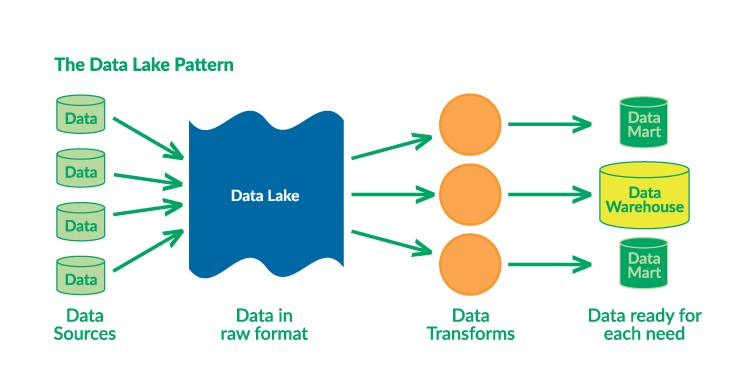
\includegraphics[width=\columnwidth]{graphics/Data.jpeg}}


\caption{Data Marts explanation.\addbibresource{bib/bib1}}
\end{figure}



\end{itemize}
\end{block}

\begin{block}{Methodologies}
\begin{itemize}
\item We include all technologies we have used in creation and functionalities of Data lake.
\item For frontend we have mainly used React, Typescript and Javascript.
\item Backend is mostly done in Python.
\item For APIs creation, usage and collection we have used Postman.
\item For storage Purpose MongoDB, Postgres and HDFS are in particular use.
\item For Deployment, Implementation and scaling Docker was used.
\item Explanation in a table:
\begin{table}
\caption{Explanatpry table for Methodologies.}
\begin{tabular}{l l l l l l}
Interface & \hspace{1em} & Technologies & \hspace{1em} & \parbox{5cm}{Purposes} \\[1cm]
\hline
Backendend\textsuperscript && Python, Java && Running functionalities\\
Frontend\textsuperscript && React, Typescript, Javascript   && Make running functionalities\\
Data Handling\textsuperscript && Apache, Docker, Postman &&  For proper data handling
\end{tabular}
\end{table}
\begin{itemize}

\end{itemize}
\end{itemize}

\vspace{0.5\baselineskip}
\begin{figure}
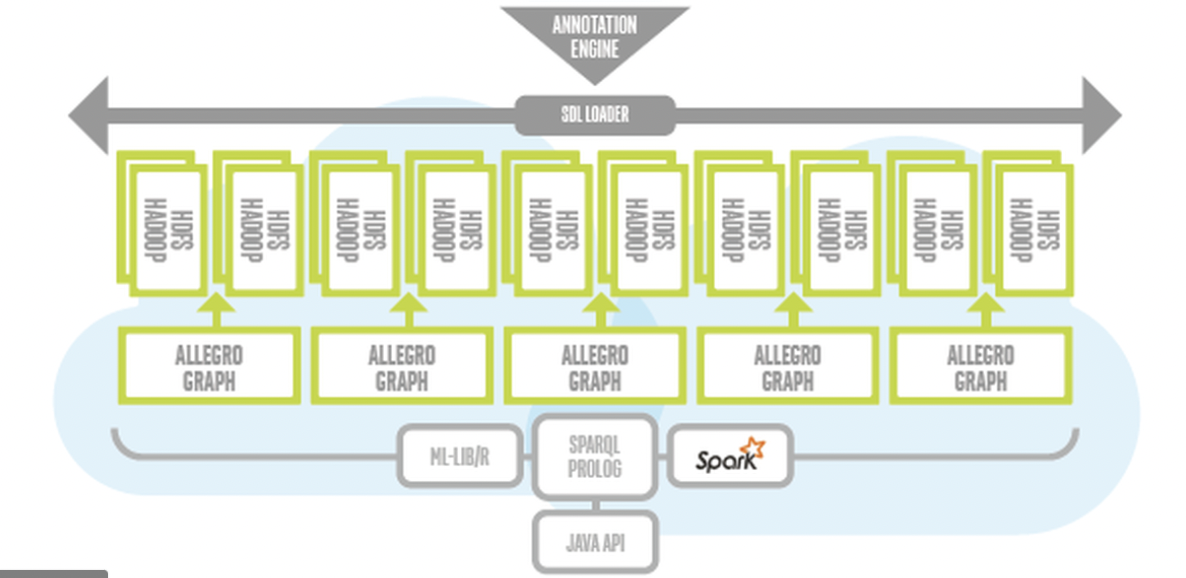
\includegraphics[width=0.99\columnwidth]{graphics/Data Lake}%

\caption{Different Layers of Data Lake. \bibliography{bib\bib2}}
\end{figure}
\end{block}


\bibliography{bib\bib2}



\end{textblock}
\begin{textblock}{0.5}(0.5, 0.00)

\begin{block}{Functionalities}
\begin{enumerate}
\item Different Ingestion Forms are used for ingestion.\\
structured (sql) and semi-structured (json, xml) data is Ingested. .\\ for each ingested dataset a metadata entry is generated ..\\
Storage.
Own: The datasets can be stored in their storage-system; For files the target storage-system  sql, postgresql, HDFS..\\ and for Database we have used  mongodb..\\
At the end there is Interaction Layer

\end{enumerate}




\begin{figure}
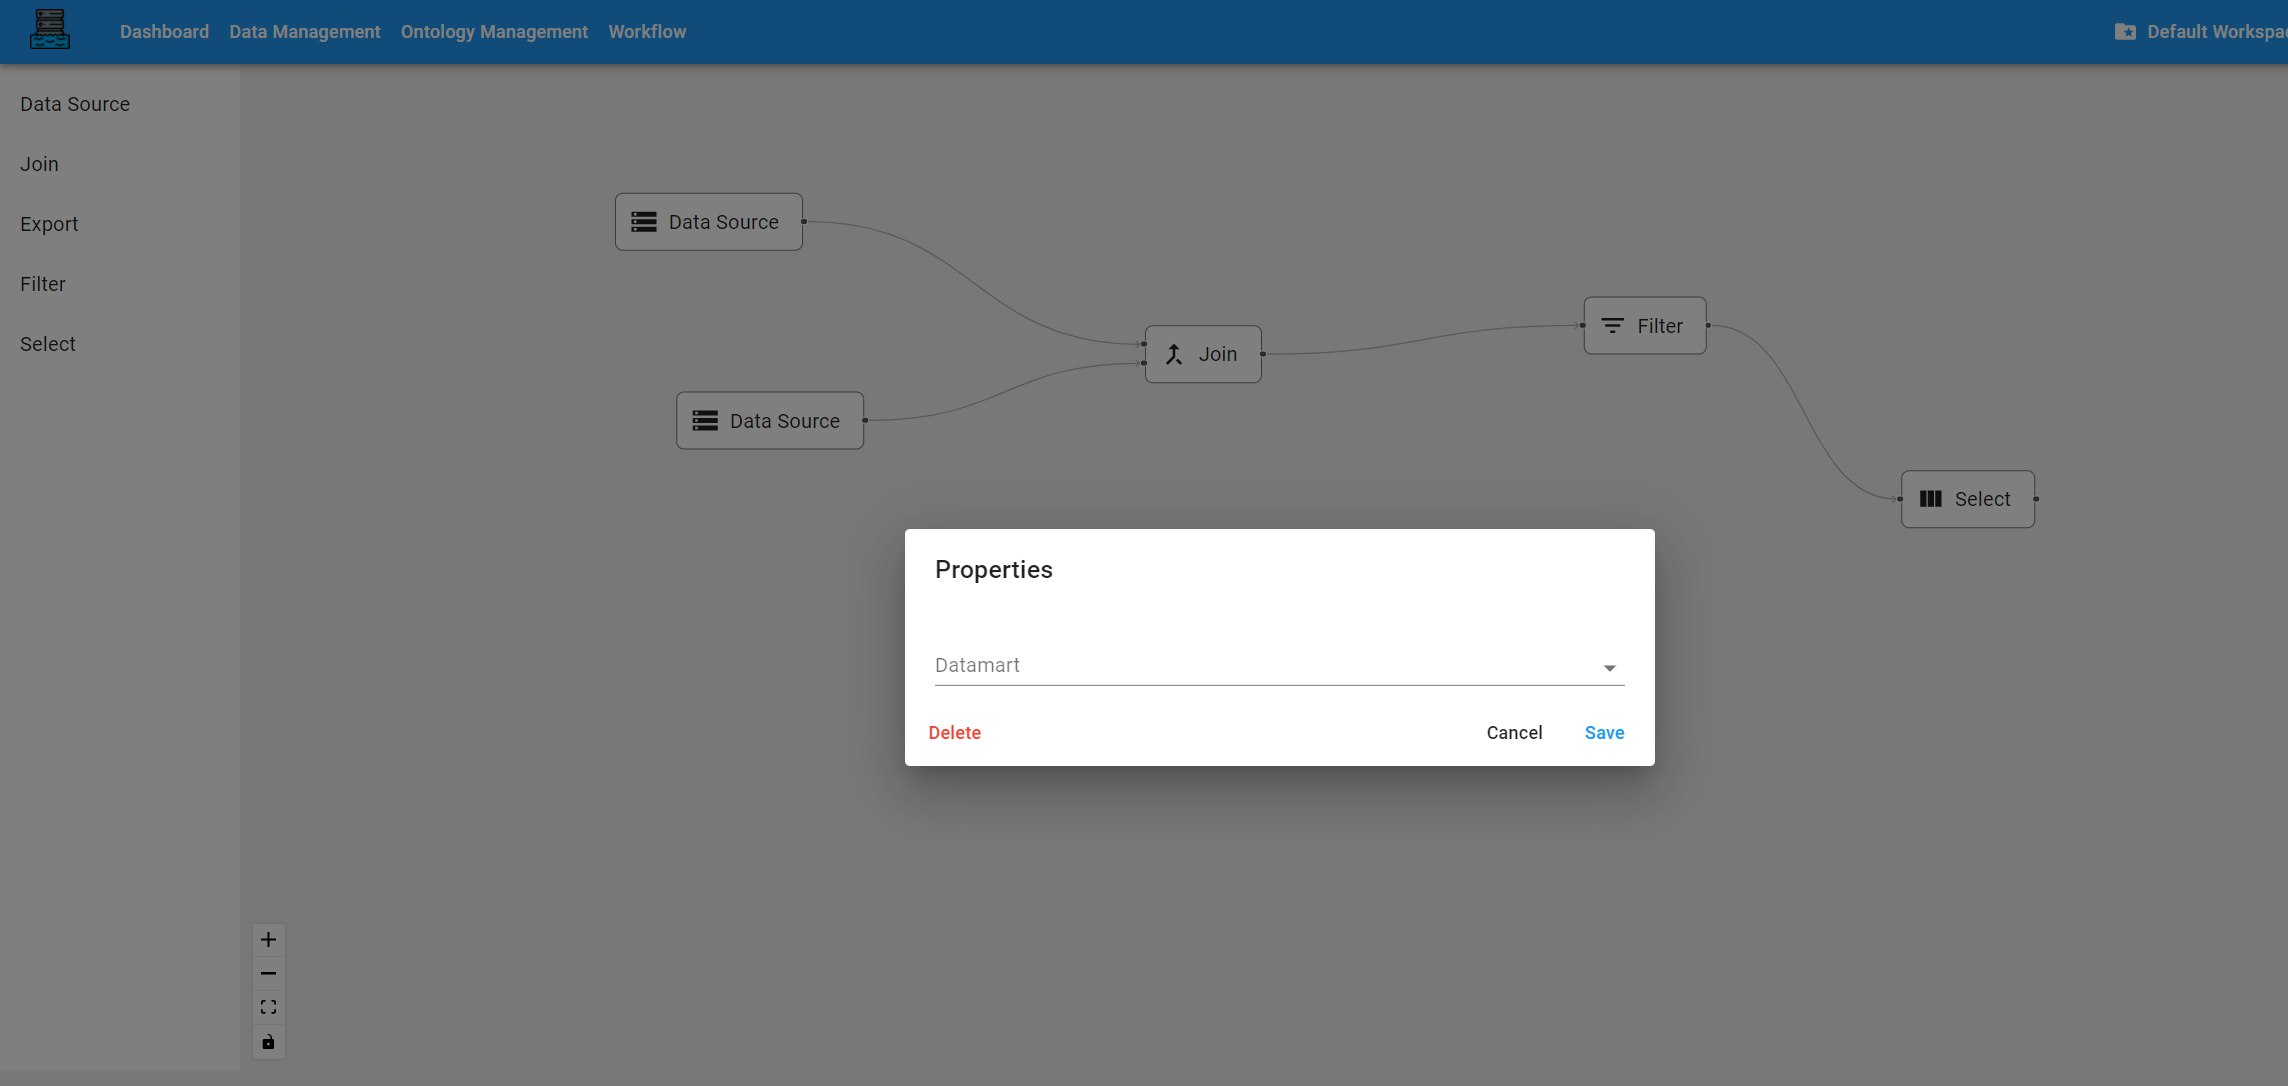
\includegraphics[width=0.99\columnwidth]{graphics/Functionality.jpeg}%

\caption{Functionality Display of Data Lake.}
\end{figure}
\end{block}

\begin{block}{ConClusion}
\begin{enumerate}
\item We have put an effort to build Masterful Data Lake. we propose it is better option to consider for handling Big Data. Continued.
\end{enumerate}
\end{block}

% the bibliography
\vfill\vspace{7.5mm} % at the bottom, but at least some spacing
\begin{block}{References}
\nocite{*}
\parbox{\textwidth}{
\AtNextBibliography{\small}
\printbibliography
}
\end{block}

\end{textblock}

\begin{textblock}{1.0}(0.0, 0.625)
\begin{figure}
%{\color{hsnrdunkelblau}\rule{\textwidth}{4pt}}
%\fbox{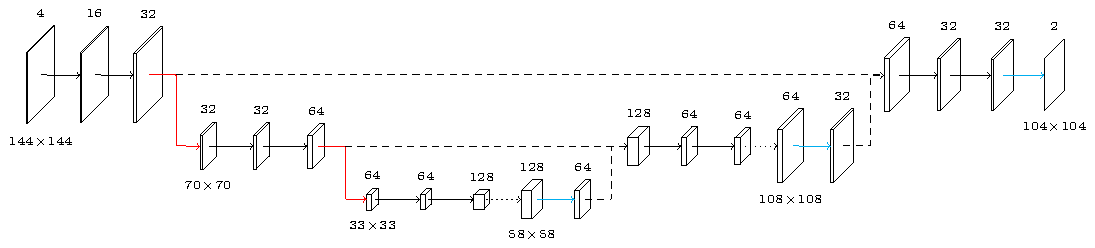
\includegraphics[width=\columnwidth]{graphics/fig_angiounet_architecture.pdf}}%
%\caption{This figure stretches across the whole width of the poster. Awesome!}
\end{figure}
\end{textblock}

\end{document}